\section[Backgroud on Quantum Metrology]
{Background on Quantum Metrology}
\thiswatermark{\put(1,-241){\color{l-grey}\rule{84pt}{48pt}}
\put(84,-241){\color{grey}\rule{410pt}{48pt}}}


\quotes{Roger J. Barlow}{In the real world, doing real experiments, statistics began to matter}

\vspace{0pt}
\lettrine[lines=2, findent=3pt,nindent=0pt]{I}{n} this chapter we will study the basics of Quantum Metrology, which stands for the science of enhanced metrology by quantum phenomena.
On the other hand, metrology, as the science of measuring, has played an essential role for the development of the technology as we know it today.
It studies several aspects of the estimation process, such as which strategy to follow in order to improve the precision of an estimation or which is the bound for the precision.
Metrology also covers all intermediate process for the estimation, from the design aspects of a precise measuring device, to the most basic concepts of estimation, which lead at the end to a better understanding of it as a whole.

In this sense, with the discovery of the Quantum Physics and the development of Quantum Mechanics, new doors for advances in metrology were open in the early decades of the 20th century.
First, Quantum Theory embraced the so-called field of Quantum Information, which merges the notions of the theory of information and computer science, among others sub-fields, with the quantum mechanics.
This new field of Quantum Information is in the basis of Quantum Metrology.
Moreover, those emerging fields rapidly became into very interesting interdisciplinary playgrounds of science attracting the interest of many scientists as well as resources for their researches.
Just to mention that the role of the so-called entanglement, an exclusive feature of Quantum Mechanics which cannot be completely described using classical probabilistic theories, is essential in this context.
With the aim of completely understand this concepts, many scientists world wide have integrated their efforts.
Said this, the entanglement also is in the center of theoretical concepts in Quantum Metrology.
In the Quantum Metrology framework, we will focus on the achievable precision of the systems.
We will show as well different strategies to achieve the desired results.

On the other hand, a very important field of science must be highlighted by its own merits.
We are mentioning the statistics, without which many descriptions of the actual and past physical findings would lack of the rigorous interpretation needed for the complexity of data samples.
It basically helps to analyse raw data to find special properties out of it.

\subsection{Background on statistics and the theory of estimation}

In this section, we will enumerate the basic concepts of statistics as well as the estimation process.
As we said, the main mathematical tools used by the metrology science belong to statistics.
Moreover, we are especially interested in estimation theory.
The statistics main characteristic is that it makes the raw data under consideration comprehensible from the human perspective.
The data can be anything, from a set of different heights of a basketball team, to the outcomes of a coin toss, or the wavelength of photons coming out of some sample.
The aim of this section is to give the reader sufficient material to follow this thesis and make it comprehensible from the beginning\footnote{
For a more detailed material, check statistics book as well as mathematics book for scientist and engineers \citep{Riley1998, BarlowXXXX}}.

\subsubsection{Probability, data samples, average and variance}

The probability indicates the relative chance of an event to happen.
For instance, if there is a box with ten red balls and five blue balls, considering that the balls of the same color are indistinguishable and that we extract one randomly, we have $\frac{5}{10+5}=\frac{1}{3}$ of probability to obtain a blue ball and $\frac{2}{3}$ to obtain a red ball.
The reader may notice many properties a probability should have, such as that the probability of any event to happen is always one or that a probability is always given by a number in between zero and one.
For more details, there are many interesting textbooks or chapters of some textbook about Probability Theory one could follow if interested.
The following References~\citep{Riley1998, BarlowXXXX} are some of those books.

When someone has a data sample at hand, it might come from diverse sources and might be represented using multiple forms such as numbers or words (for instance, a table of names of people), the first thing one tries to accomplish is to analyze the data to extract the relevant properties from it.
A data sample always come from a population sample, i.e., the data sample might not be complete (one could lose some in the process) neither exact (a measuring device always have an error when estimating a magnitude).
Hence, the data sample comes attached with a probability for each data element.
In the subsequent paragraphs, we will describe this relation and we will enumerate the most useful properties and formulas for the comprehensions of this thesis.

First of all, we will explain our notation which follows the one used on Reference~\citep{Riley1998}.
A probability function gives the probability of an event $x$ to happen when measuring some random variable $X$, and it is denoted by $\prob(X=x)$.
Second, the $N$ elements of a data sample are considered to come from $N$ random variables with the corresponding $N$ values due to the random nature of the measuring, $\{X_i=x_i\}_{i=1}^N$.
The joint probability of those random variables is in general not separable.
This is due to the fact that the outcomes could depend on the rest of the outcomes or some other more complex relation that makes the most general case to be non-separable from the probabilistic point of view.
Therefore we define this PDF as an $N$ variable function
\be
  \prob(\bs{X}=\bs{x}) \equiv \prob(X_1=x_1,X_2=x_2,\dots,X_N=x_N).
\ee
If separable this is written by
\be
  \prob(\bs{X}=\bs{x}) = \prod_{i=1}^N\prob(X_i=x_i)
\ee
and it is the case for many relevan cases.

When some property of the system is defined as a function of random variables, the result is also a random variable with another transformed PDF.
For example, we measure the position of a body at some moment.
If the system was at rest on the origin at initial time and the acceleration is known to be constant, then from the position one can infer on the value of the acceleration by using $A=2X/t^2$, where $X$ denotes the position at instant $t$ and $A$ the acceleration.
If $X$ is a random variable, which is the general case when measuring the position of a body, then the probability is computed in this case by
\be
  \prob(A=a) = \frac{\text{d}x}{\text{d}a}\prob(X=x)=\frac{2}{t^2}\prob(X=x).
\ee
In general for the multiple random variable case transformations, we must require that
\be
  |\prob(\bs{X}=\bs{x})\,\text{d}x_1\text{d}x_2\dots\text{d}x_N|=|\prob(\bs{Y}=\bs{y})\,\text{d}y_1\text{d}y_2\dots\text{d}y_N|.
\ee
This leads to some interesting formulas we will discuss later.

We now stick to the simplest case on which the data is a collection of values of the same random variable describing the same physical one-dimensional data population.
Some definitions reasonable to mention in this thesis arise for those kind of data samples: the average, variance, moments and central moments.
The arithmetic average (there are other types of average one can find in the textbooks) is computed by
\be
  \overline{x}=\frac{1}{N}\sum x_i.
\ee
The variance is related with the spread of the data and computed by
\be
  \sigma^2=\frac{1}{N}\sum (x_i-\overline{x})^2,
\ee
where $\sigma$ is the standard deviation.
Different moments are computed by $\overline{x^r}=\frac{1}{N}\sum x_i^r$ while central moments are of the form of $n_r=\frac{1}{N}\sum (x_i-\overline{x})^r$.
Notice that the variance is the second central moment of the data sample.
For completeness, when each element of the data consists of more than a number, e.g., $(x_i,y_i,z_i)$, the co-variance between two data kinds, in the following case $X$ and $Y$, is obtained by
\be
  V_{X,Y} = \frac{1}{N}\sum_{i=1}^N (x_i-\overline{x})(y_i-\overline{y}).
\ee

Those functions also apply to the probability distribution functions.
While these last ones may be unknown functions for us, as soon as we collect all the possible data or we are in the large number regime the variances of the data sample and of the data population, the means, the co-variances and so on so forth, they must coincide.
We will try to keep this distinction as clear as possible.
In general the mean values of any function over data sample values $g(x)$ are denoted with a bar over a lowercase variable, e.g., $\overline{x^r}$ for the $r$-th moment, while the mean values of any function applied to the data population $g(X)$ is written following some textbooks by $\text{E}[g(X)]$.
One clearly may distinguish two cases here: one for continuous functions where the expectation values or the means are computed integrating over all the possible values, and the other case on which $\prob(\bs{X}=\bs{x})$ can take only discrete values.
For completeness here are the two definitions
\be
  \text{E}[g(\bs{X})] = \lcor
  \begin{split}
    &\int g(\bs{x}) \prob(\bs{X}=\bs{x})\,\text{d}^N \bs{x},\\
    &\sum_{i,j,\dots} g(\bs{x}) \prob(\bs{X}=\bs{x}).
  \end{split}
  \right.
\ee
One more definition needs our attention and it is the variance any function $g(X)$ denoted by $\text{V}[g(X)] \equiv \text{E}[g(X)^2] - E[g(X)]^2$.

\subsubsection{Frecuentist vs. bayesian approach}

\subsubsection{Estimators and Fisher information}

Let us suppose that the data sample has encoded some wanted parameters $\bs{a}\equiv(a_1,a_2,\dots)$.
The underlying probability, in general also unknown, may be conditioned by the real values of the wanted parameters $\bs{a}$.
The probability of the data sample is therefore written as
\be
  \prob(\bs{X}=\bs{x}|\bs{a}),
\ee
where "$|\bs{a}$" indicates its dependency on these parameters.
At this point, notice that an estimate of the the wanted parameter based on the data sample has the form of a function the random variables.
Therefore as mentioned before, an estimator of $a$, which is how is called this quantity and is denoted by $\hat{a}$, is another random variable with a PDF of the form of
\be
  \prob(\hat{a}|\bs{a})\,\text{d}\hat{a} = \prob(\bs{X}=\bs{x}|\bs{a})\,\text{d}x_1\text{d}x_2\dots\text{d}x_N.
\ee
For short, we omit on writing $\bs{X}$ from now on, thus the conditional joint probability of $N$ random variables is written as $\prob(\bs{x}|\bs{a})$.

As we said, an estimator is defined to be a function of the data sample.
For example, one of such estimators is the estimator of the mean value of the data population, in general unknown.
The mean value of the data population, which in general we do not have access to, is denoted usually by $\mu$.
Notice that $\mu$ is in general different from the mean value of the data sample $\overline{x}$.
A valid estimator for the population mean value would be the arithmetic mean of the data sample, i.e., $\hat{\mu}=\overline{x}$.

An important notion of an estimator is its \emph{efficiency}, i.e., whether it has smaller variance than another.
The more efficient estimator the smaller variance it has.
Remember than an estimator is a random variable so it must have a variance that comes from the data population, i.e., from $\prob(\hat{a}|\bs{a})$ in this case.

For an estimator of any kind there is a theoretical lower bound for its variance.
For the proof of the previous observation, which we compute for continuous random variables without losing of generality, we start with the normalization of the PDF
\be
  \int \prob(\bs{x}|\bs{a})\,\text{d}^N\bs{x} = 1.
\ee
Next, we compute the partial derivative over $a$ such that
\be
  \int \partial_a\prob(\bs{x}|\bs{a})\,\text{d}^N\bs{x} = \int \partial_a\big(\ln  \prob(\bs{x}|\bs{a})\big) \prob(\bs{x}|\bs{a}) \,\text{d}^N\bs{x} = 0,
\ee
where for simplification, we omit the arguments of the joint probability on the second equality.
From Eq.~\eqref{}, it turns out that the Eq.~\eqref{} is the expectation value of $\partial_a(\ln\prob)$.
Finally if we have an unbiased estimator, for which the true value $a$ coincides with the expectation value of the estimator $\text{E}[\hat{a}]$, its partial differentiation over $a$ must be equal to one,
\begin{align}
  \partial_a\text{E}[\hat{a}] &= \partial_a a = 1, \\
  \begin{split}
    1 &= \partial_a \int \hat{a} \prob(\bs{x}|\bs{a})\,\text{d}^N\bs{x} \\
      &=  \int \hat{a} \partial_a\prob(\bs{x}|\bs{a})\,\text{d}^N\bs{x} =  \int \hat{a} \partial_a\big(\ln  \prob(\bs{x}|\bs{a})\big) \prob(\bs{x}|\bs{a}) \,\text{d}^N\bs{x},
  \end{split}
\end{align}
where we apply the definition of the expectation value of the estimator $\hat{a}$ for continuous variables and we apply as well similar identities as in Eq.~\eqref{}.

At this point we invoke the Schwartz inequality for two real multidimensional functions $g(\bs{x})$ and $h(\bs{x})$ such that $(\int g h \,\text{d}^N\bs{x})^2\leq (\int g^2 \,\text{d}^N\bs{x}) (\int h^2 \,\text{d}^N\bs{x})$.
With this we can follow the following recipe to obtain a lower bound for the variance of a general estimator.
First the definition of the variance looks like
\be
  V[\hat{a}] = E[(\hat{a}-a)^2] = \int (\hat{a} - a)^2\prob(\bs{x}|\bs{a})\,\text{d}^N\bs{x}.
\ee
Second, from Eqs.~\eqref{,} holds that
\be
  \int (\hat{a}-a)\partial_a\big(\ln  \prob(\bs{x}|\bs{a})\big) \prob(\bs{x}|\bs{a})\,\text{d}^N\bs{x} = 1
\ee
because $a$ is not a function of $\bs{x}$.
Hence, using the Schwartz inequality we can write
\be
  \text{V}[\hat{a}] = \int (\hat{a} - a)^2\prob(\bs{x}|\bs{a})\,\text{d}^N\bs{x} \geq \frac{1}{\int \lcua\partial_a\big(\ln \prob (\bs{x}|\bs{a}) \big)\rcua^2 \prob (\bs{x}|\bs{a})\,\text{d}^N\bs{x}},
\ee
which is also known as the Cram\'er-Rao bound or the Fisher inequality.
The denominator on the right hand-side is called generally the Fisher information (FI).

With this review of the most interesting features of "classical" metrology, from the point of view of this thesis, we conclude this section.
In the next section, we will record some properties of the Quantum Mechanics and then we will follow with another s with the basis of Quantum Metrology.

\subsection{Quantum Mechanics from metrology perspective}

The ubiquitous probabilistic nature of Quantum Mechanics forces us to use probabilities on a regular basis.
Moreover, if one works on fields connected with experiments or some short of physical realizations this probabilistic nature of Quantum Mechanics is enhanced.
On the other hand, exotic features such as entanglement arise from Quantum Mechanics, which give us unique opportunities to exploit them as resources.
The present section is intended to describe these quantum phenomena in more or less detail.

\subsubsection{The quantum state, multiparticle state, entanglement}

A formal mathematical description of the quantum state is given next.
This also allows us to introduce some notation used through the thesis.
A \emph{state} in Quantum Mechanics lives on a Hilbert space, $\mathcal{H}$.
The system state, $\rho$, has the following properties:
\begin{enumerate}
  \item
  It is Hermitian, so it is invariant under the complex transposition, $\rho=\rho^\dagger$ and all its eigenvalues are real.
  \item Its trace is equal to one, $\tr(\rho)=1$.
  \item It is positive semi-definite, i.e, all its eigenvalues are bigger or equal to zero, $\rho=\sum_{\lambda}p_\lambda \Pi_\lambda$ where $p_\lambda\geq 0$ and $\Pi_\lambda\equiv\ketbra{\lambda}{\lambda}$ is the projector of the eigenstate $\ket{\lambda}$.
  From (ii), it follows that $\sum_\lambda p_\lambda = 1$.
  \item If all $p_\lambda$ are zero except one, the state is called a pure state and is equivalent to the projector of such eigenstate $\rho=\Pi_\lambda\equiv\ketbra{\lambda}{\lambda}$, where $\ket{\lambda}$ denotes a pure \emph{vector} state.
  \item It follows that the quantum states form a convex set where the extreme points are pure states.
\end{enumerate}

The composite system of $N$ different parties live in the Hilbert space $\mathcal{H} = \mathcal{H}^{(1)}\otimes\mathcal{H}^{(2)}\otimes\cdots\otimes\mathcal{H}^{(N)}$ or for short $\mathcal{H} = \bigotimes_{i=1}^N\mathcal{H}^{(i)}$, where $\otimes$ stands for tensor product.
For instance, this composite Hilbert space could be used to represent a many-particle system, in this case $N$ particles.
A \emph{separable} state in this Hilbert space can be described by
\be
  \label{eq:bg-separable-state-definition}
  \rho_{\text{sep}} = \sum_{i}p_i\rho_i^{(1)}\otimes\rho_i^{(2)}\otimes\cdots\otimes\rho_i^{(N)},
\ee
where $p_i$ are convex weights that sum to one and are equal or bigger than zero.
If not the state is said to be \emph{entangled}.
We mention it as a formal description of the entanglement \citep{}.
One may notice at this moment, that relaxing the requirements of Eq.~\eqref{eq:bg-separable-state-definition}, one can lead to different classifications of the states.
Concepts like genuine multipartite entanglement, $k$-producible states, or entanglement depth, among others, arose from weakelly constrain the Eq.~\eqref{eq:bg-separable-state-definition} \citep{}.

It is important to remark one of such classifications in order to characterize the different levels or multipartite entanglement followed in this work.
We call a state $k$-producible, if it \emph{can} be written as a mixture of the tensor product of different multiparticle states with at most $k$ particles,
\be
  \rho_{k\text{-pro}} = \sum_i p_i\rho^{(\alpha,\dots,\beta)}_i \otimes \rho^{(\gamma,\dots,\delta)}_i\otimes \dots,
\ee
where superscript indexes between parenthesis go from 1 to $N$ and denote to which parties belong the state, and where each index appears once in each sum element.
If a state cannot be written as $k$-producible, then it must be $(k+1)$-entangled.
This defines the entanglement depth.
Later on those concepts will arise on the metrology framework \citep{,}.

Besides those concepts, we present a set of operators that will appear many times in all chapters, namely the angular momentum operators.
Again those definitions allow us to introduce notation used on this book.
For a single party with discrete $d$ levels and therefore $s=(d-1)/2$, the eigenvalue equation for the angular momentum projection operators are
\be
  j_l^{(n)}\ket{m}_l^{(n)} = m \ket{m}_l^{(n)}
\ee
for $m=-s,\dots,+s$,  where $l=x,y,z$ and where it is usual to omit the subscript and superscript, $l$ and $(n)$ respectively, for simplicity.
The square of the total angular momentum, $\bs{j}^2=j_x^2+j_y^2+j_z^2$, for a single party is simply
\be
  (\bs{j}^2)^{(n)}\rho^{(n)}=s(s+1)\rho^{(n)},
\ee
where $\rho^{(n)}$ is an arbitrary pure or mixed state defined on the $\mathcal{H}^{(n)}$ Hilbert space.

The collective angular momentum projection operators are defined as the sum of their respective single-party spin operators such that they are extended to the rest of the Hilbert spaces by tensor products of the identity operators defined for the rest of subspaces,
\be
  J_l = \sum_{i=1}^N \mtxid^{(1,\dots, i-1)} \otimes j_l^{(i)} \otimes \mtxid^{(i+1,\dots,N)} \equiv \sum_{i=1}^1 j_l^{(i)},
\ee
where $\mtxid$ stand for the identity operator and the last formula is the most used since it is easy to notice that the single subspace operator must extended in each case.
The square of the angular momentum projections of a many-particle system is not equal to the sum of the square angular momentum projection of each of the parties and it is obtained by
\be
  J_l^2 = \sum_{i,j}^N j_l^{(i)} j_l^{(j)} = \sum_{i=1}^N (j_l^2)^{(i)}+\sum_{i\neq j}^N j_l^{(i)} j_l^{(j)}.
\ee
Therefore, the total square angular momentum is neither the sum of all single-party square angular momentum and is computed by
\be
  J_l^2 = \sum_{i,j}^N j_l^{(i)} j_l^{(j)} = \sum_{i=1}^N (j_l^2)^{(i)}+\sum_{i\neq j}^N j_l^{(i)} j_l^{(j)},
\ee
where we separated the sum into two pieces, the first corresponds to the sum of all single party angular momentum projections squared and the second corresponds to the product of angular momentum projection operators of two distinct subsystems.
Many more combinations of these single-party operators may arise on different contexts.
In the Appendix~\ref{}, we discuss in more detail the different structures that arise from adding the angular momentum operators, e.g., the symmetric subspace or the fixed total angular momentum subspace.

Evolution:

- Markov

- Limblad

Measurements:

- POVMs

Quantum Information:

\subsection{Quantum Metrology}

We summarize important recent advances in Quantum Metrology
Simple metrological setups allow for encoding some wanted parameter into the state of the system, thus from the readout of the final state one can infer on it.
The estimation theory applied to the intrinsic probabilistic nature of quantum states has lead to the the formulation of Quantum Metrology.
Merging the probabilistic features of quantum mechanics and the estimation theory is not trivial.
Nevertheless, starting from the pioneering works of Wotters, Braunstein and others back in 19XX \citep{}, until the works of Giovannetti et al, Paris and others roughly 20 years later \citep{}, the field of Quantum Metrology has been stabilized with solid foundations.
Later, advanced works in Quantum Metrology appeared \citep{} together with experimental realizations \citep{} which raised the interest in this topic.
In this section, we will highlight the most important aspects of this field and with this we will conclude this introductory chapter.

\subsubsection{Quantum Magnetometry}
\label{sec:bg-quantum-metro}

Without losing of generality, one of the most basic tasks of Quantum Metrology is to address the \emph{precision} of estimating some unknown magnetic field strength, namely $B$, based in the interaction with the system.
In this section we will assume that the magnetic field is homogeneous on the position space.
To consider more advanced situations on which the magnetic field changes linearly with the position, see chapter [XXX].
With the aim of estimating the strength of the magnetic field, a prove state is used in order to interact with it, coupling the magnetic moment of the state and the field itself.
After some time, the state has evolved.
Finally, measuring how the state has changed one would be able to infer on the strength of the magnetic field, basically proportional to the change on the state.

In general, we will say that the magnetic moments of the states come exclusively from the spin angular momentum, neglecting any possible contribution from the orbital angular momentum.
This way the physics is simpler.
This is justified in the sense that most of the recent experiments on this context have been carried out with ion-traps, BECs or at most cold atomic ensembles, which have indeed a negligible orbital angular momentum.

Beside this considerations, the interaction Hamiltonian can be written as,
\be
  H = - \bs{\mu} \cdot \bs{B}
\ee
up to some constant factor.
Now in the simplest case we will choose the magnetic field to be pointing to some fixed direction, for instance, the $z$-direction.
So the magnetic field vector can be written as ${B}=B\bs{k}$, where $\bs{k}$ is the unitary vector pointing to the $z$-direction.
This way estimation problem is much more simple, since one has not to determine the direction of the magnetic field.

The magnetic moment of the system is proportional to the spin angular momentum, $\bs{\mu}=-\mu_\text{B} g_{\text{s}}\hbar^{-1} \bs{J}$, where $\mu_{\text{B}}$ and $g_{\text{s}}$ are the Bohr magneton and anomalous gyromagnetic factor respectively.
Finally, one can rewrite the interaction Hamiltonian as,
\be
  H = \gamma B J_z
\ee
where $\gamma = \mu_\text{B} g_{\text{s}}\hbar^{-1}$ and we have used the fact that $\bs{J}\cdot\bs{k}=J_z$.
Finally, the unitary operator leading the evolution of the system can be written as,
\be
  U = \exp(-i\Theta J_z),
\ee
where the magnetic field strength is encoded into the variable $\Theta=-\mu_\text{B} g_\text{s} t B/\hbar$.
Here $\mu_\text{B}$ stand for the Magneton of Bhor and $g_\text{s}$ for the giro-magnetic constant for the spin angular momentum, and $t$ is the time spent on the evolution.

\begin{figure}
  \centering
  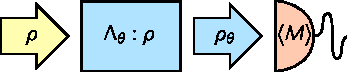
\includegraphics[scale=.85]{img/BG_preparation_encoding_estimation.pdf}
  \caption[Quantum Metrology estimation process]{Secuence of the different steps for the basics of the estimation process on Quantum Metrology. First, an input state $\rho$ enters the region on which the unknown parameter $\Theta$ is imprinted on it, for the most general case, representented with $\Lambda_{\Theta}$. Last, the state that has encoded the parameter $\Theta$ on it is measured and $\Theta$ must be infered from the measured quantity $\expect{M}$.}
  \label{fig:bg-preparation-encoding-estimation}
\end{figure}

\begin{figure}
  \centering
  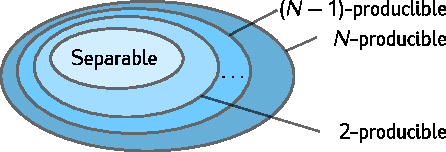
\includegraphics[scale=.85]{img/BG_separability_k_producibility_circle.pdf}
  \caption[Diagram for $k$-producibility sets]{}
  \label{fig:bg-separability-k-producibility-circle}
\end{figure}

\be
  \label{eq:bg-pezze-bound}
  \qfi[\rho,J_z] \geq \frac{\expect{J_y}^2}{\varian{J_x}}
\ee
